\documentclass{beamer}

\title{Student wellbeing survey web application}
\author{Tarnjot Singh Virdee (24009864)}

\usetheme{Pittsburgh}

\begin{document}

\maketitle

\begin{frame}
\begin{columns}
    \column{.4\textwidth}
    \begin{itemize}
        \item 15\% to 20\% of youth suffer from some mental health issues
        \vspace{.2cm}
        \item 95\% of youth own a smartphone
    \end{itemize}

    \column{.6\textwidth}
    \includegraphics[height=1\textheight]{images/Mental-Health-1.jpg}

\end{columns}
\end{frame}

\begin{frame}
    \frametitle{Motivation}
    \begin{itemize}
        \pause
        \item Help students track their own wellbeing 
        \pause
        \vspace{.2cm}
        \item Potentially improve it too 
        \pause 
        \vspace{.2cm}
        \item Anonymity removes potential shame
    \end{itemize}  
\end{frame}  

\begin{frame}
    \frametitle{Current solutions}
    \begin{columns}
        \column{.5\textwidth}
        \includegraphics[height=.35\textheight]{images/Google-Surveys-logo.png}
        \includegraphics[height=.35\textheight]{images/2017-surveymonkey-new-logo-design-4.png}

        \column{.5\textwidth}
        \begin{itemize}
            \pause
            \item Very generic 
            \pause
            \vspace{.2cm}
            \item Aimed at covering as many use cases as possible
            \pause
            \vspace{.2cm} 
            \item Unable to produce tailored feedback
        \end{itemize}
    \end{columns}
\end{frame}

\begin{frame}
    \frametitle{Proposed solution} 
    \begin{columns}
        \column{.4\textwidth}
        \includegraphics[width=1\textwidth]{images/icon-actions.png}
        
        \column{.6\textwidth}
        \begin{itemize}
            \pause
            \item Create scorable surveys 
            \pause
            \vspace{.2cm}
            \item Students can build up a score history
            \pause
            \vspace{.2cm}
            \item Track wellbeing based on that
            \pause
            \vspace{.2cm}
            \item Score decides what resources they get referred to
        \end{itemize}
    \end{columns}
    

\end{frame}

\begin{frame}
    \frametitle{Technical specification}
    \begin{columns}
        \column{.3\textwidth}
        \includegraphics[width=.8\textwidth]{images/server_to_client.png}
        \includegraphics[width=.7\textwidth]{images/api_icon.png}
        \column{.7\textwidth}
        \begin{itemize}
            \pause
            \item Server side application 
            \begin{itemize}
                \item Manage databases
                \item Provide an API for client
            \end{itemize}
    
            \pause
            \vspace{.2cm}
            \item Client side application 
            \begin{itemize}
                \item Consumes the API
                \item Provide the necessary functionality
                \item Fast, simple to use
                \item Reusable code for future mobile app
            \end{itemize}
    
            \pause
            \vspace{.2cm}
            \item Allow for future scalability
        \end{itemize}    
    \end{columns}

\end{frame}

\begin{frame}
    \frametitle{High level architecture}
    \begin{columns}
        \column{.5\textwidth}
        \includegraphics[height=.75\textheight]{images/simple_solution_architecture.png}

        \column{.5\textwidth} 
        \begin{itemize}
            \pause
            \item Server running a Java SpringBoot application
            \begin{itemize}
                \item Provides a collection of REST API endpoints
            \end{itemize}
            
            \pause
            \vspace{.2cm}
            \item REACTjs front end client
            \begin{itemize}
                \item Uses the API to provide the necessary functionality
            \end{itemize}

            \pause
            \vspace{.2cm}
            \item Serves user requests
        \end{itemize}
    \end{columns}    
\end{frame}

\begin{frame}
    \frametitle{Security}
    \begin{columns}
        \column{.6\textwidth}
        \begin{itemize}
            \pause
            \item Oauth2 based authentication
            \begin{itemize}
                \item Secure resources exposed by API
                \item Issue tokens to client
            \end{itemize}

            \pause
            \vspace{.2cm}
            \item Json Web Tokens
            \begin{itemize}
                \item No need to manage sessions
                \item Increases scalability
            \end{itemize}

            \pause
            \vspace{.2cm}
            \item Bcrypt password encryption
            \begin{itemize}
                \item 10 rounds of encryption
            \end{itemize}
        \end{itemize}

        \pause
        \column{.5\textwidth}
        \includegraphics[height=.7\textheight]{images/simple_auth_flow.png}
    \end{columns}
    

\end{frame}

\begin{frame}
    \frametitle{Technologies overview}
    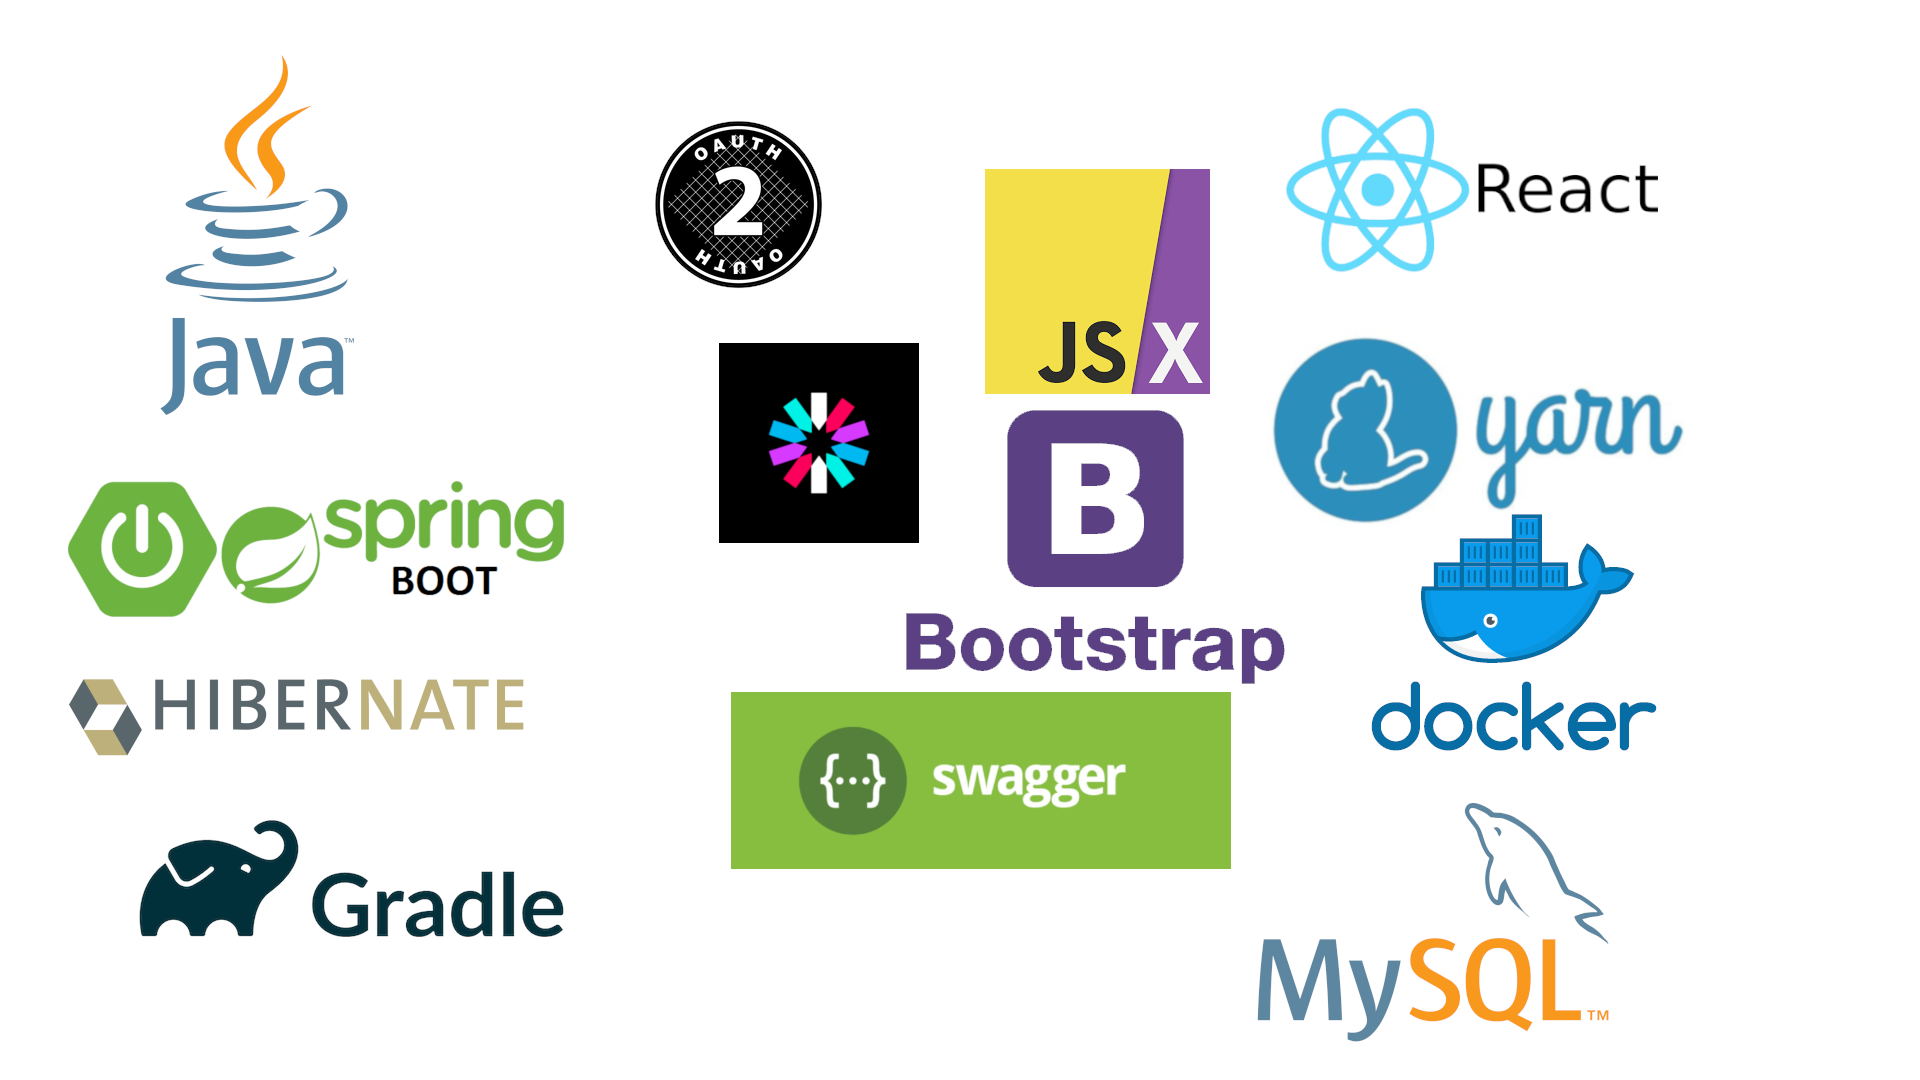
\includegraphics[width=1.1\textwidth]{images/logo_splash.png}
\end{frame}
\end{document}